\chapter{REDE NEURAL \& TRANSPORTE DE VALE}
No capítulo \ref{cap:redesneuraisempoucaspalavras} foram explicados os principais conceitos relacionados a redes neurais e como estes afetam o treinamento. Como explicado na introdução, as redes neurais podem ser treinadas para diversas tarefas específicas. O objetivo deste trabalho é encontrar modelar uma RNA que seja capaz de aprender a relação entre as configurações físicas de uma nanofita de grafeno, a energia imposta sobre ela e a transmissão de vale. Dessa forma, espera-se que a RNA seja capaz de determinar a transmissão de vale para configurações de nanofitas de grafeno não conhecidas pela RNA. 
Este objetivo pode ser modelado como um problema supervisionado de regressão numérica, mais especificamente uma aproximação de função \cite{cybenko1989approximation, hornik1989multilayer} cujas entradas são as configurações da nanofita de grafeno e energia e cuja saída seja a transmissão de vale. Considerando as entradas como um vetor \textbf{$x$} e a saída como \textbf{$d$}, tem-se:
\begin{equation*}
    d=f(x)
\end{equation*}
Um conjunto de dados de treinamento $T$ contendo os valores conhecidos de transmissão de dados e as configurações da nanofita de grafeno é dado, portanto tem-se:
\begin{equation}
\label{eqn:conjuntoTreinamento}
    T = {(x_i,d_i)}^N_{i=1} 
\end{equation}
Finalmente espera-se que a função $F(x)$ seja dada pela RNA e que descreva o mapeamento entrada-saída próximo o bastante de $f(x)$ no que diz respeito ao espaço euclidiano sobre todas as entradas, portanto tem-se:
\begin{equation*}
    ||F(x) - f(x)|| < \epsilon \text{ para todo } x
\end{equation*}
onde $\epsilon$ é um número positivo pequeno uma vez que $T$ é grande o bastante e que a rede é configurada com adequados hiperparâmetros.
A habilidade de uma rede neural de aproximar um mapeamento desconhecido entrada-saída pode ser analisado de duas formas:

\begin{itemize}
    \item Identificação de sistema: Usando o conjunto de treinamento \ref{eqn:conjuntoTreinamento} e dado que $y_i$ o vetor de saída para o vetor de entradas $x_i$, treina-se uma rede neural que minimiza o erro ($\epsilon$) dada a diferença dos quadrados entre $d_i$ e $y_i$ e ajusta os seus parâmetros livres (pesos e biases) de acordo com o $\epsilon$ encontrado na computação de todo o conjundo de treinamento $T$.
    \item Modelagem inversa: Quando deseja-se construir um \textit{modelo inverso} que produz o vetor \textbf{$x$} em resposta a um vetor $d$. O sistema inverso pode ser descrito por:
    \begin{equation*}
        x=f^{-1}(d)
    \end{equation*}
    Onde $f^{-1}(.)$ detona o inverso da função $f(.)$. Em muitas situações $f^{-1}(x)$ não é uma função facilmente calculável e por isso o uso de RNA se faz necessário, pois com ela espera-se encontrar uma aproximação de $f^{-1}(.)$. Neste caso, o vetor de entrada é $d_i$ e o vetor $x_i$ é tratado como resposta esperada. Da mesma maneira que em \textit{Identificação de sistema}, o $\epsilon$ é erro usado para ajustar os parâmetros livres da RNA a qual tenta minimizar a diferenças dos quadrados entre as saídas do sistema inverso desconhecido e a RNA. Tipicamente \textit{Modelagem Inversa} é uma tarefa de aprendizado mais difícil que \textit{Identificação de sistema} uma vez possivelmente não haja apenas uma única solução.
\end{itemize}

A seguir serão apresentadas algumas técnicas que facilitam a fase de treinamento tornando o processo de aprendizado mais rápido.

\section{Heurísticas para uma melhor performance do algoritmo de retropropagação}
Dizem que fazer o design é mais uma arte do que ciência. Isso acontece porque o resultado depende muito das experiências das pessoas, do conjunto de dados etc. Em parte isso é verdade, porém há algums métodos que ajudam uma rede neural a ter melhor performance. Abaixo serão explicados os métodos e fatores que influenciaram no experimento de treinar uma rede neural capaz de predizer o transporte de vale em nanofitas de grafeno deformada por gaussianas.

\subsection{Atualização em batch (lote) versus atualização estocástica}
O modo estocástico (sequencial) implica que os pesos sinápticos da rede neural são atualizados de acordo com cada exemplar do conjunto de treinamento. Ele é computacionalmente mais rápido que o modo em batch principalmente quando o conjunto de treinamento é grande e redundante, ou seja, que possui exemplares repetidos. Dados altamente redundantes acabam deixando o cálculo da matriz Jacobiana (necessária para atualização em lote) mais complexo.

\subsection{Conjunto de treinamento com máxima informação}
Como regra geral, todo exemplar de treinamento apresentado ao algoritmo de retropropagação deve ser escolhido com base na quantidade máxima de informação possível para o treinamento em questão (LeCun, \citeyear{lecun1993efficient}). Há duas maneiras de fazer isso:

\begin{itemize}
    \item Usar um exemplar que resulte no maior erro de treinamento.
    
    \item Usar um exemplar que seja radicalmente diferente de todos os outros previamente apresentados ao algoritmo.
\end{itemize}

Essas duas heurísticas são motivadas pelo desejo de se ter uma maior busca no espaço de pesos. Um método simples e comumente usado é ordenar de forma aleatória o conjunto de treinamento de forma a minimizar as chances de que exemplares similares sejam apresentados ao algoritmo. 

\subsection{Função de ativação}
No que diz respeito a velocidade de aprendizado, é preferível usar uma função de ativação do tipo sigmoid e que seja impar ao seu parâmeto, ou seja $\phi(-x)=-\phi(x)$. A função tangente hiperbólica, com as constantes $a=1.7159$ e $b=\frac{2}{3}$  satisfaz essa característica pois $\phi(1)=1$ e $\phi(-1)=-1$. Além disso, conforme mostrado abaixo, o ganho efetivo da função de ativação é próximo de $1$:

\begin{align*}
\phi(0) = & ab \\
= & 1.7159 \frac{2}{3} \\
= & 1.1424        
\end{align*}

\subsection{Atributos a serem preditos}
Os atributos a serem preditos, ou seja, a(s) saída(s) da rede neural precisam evitar os limites da função de ativação escolhida. Caso contrário, os pesos sinápticos tendem ao infinito diminuindo assim o processo de aprendizado ao colocar os neurônios das camadas ocultas em saturação. Como alternativa a usar a função de ativação com valores específicos citados acima para as constantes $a$ e $b$ da função de ativação, é sugerido pré-processar os dados de forma que evitem o limites, ou seja, a(s) resposta(s) desejada(s) da rede neural pode(m) estar compreendida(s) no intervalo [-0.9, 0.9]

\subsection{Normalização das entradas da rede neural}
Cada variável de entrada deve ser préprocessada de forma que sua média, ponderada sobre todo o conjunto de dados, seja próxima de zero ou que seja pequena se comparada a seu desvio padrão (LeCun,  \citeyear{lecun1993efficient}). Isso garante que os pesos na(s) camada(s) oculta(s) evitem a oscilação de direção na superfície de erro, acelerando assim o processo de aprendizado.

Além disso, as variáveis de entrada, se possível, não devem estar correlacionadas conforme mostrado na figura \ref{fig:correlacao}, onde é possível observar que exceto por a variável \textit{Transmissão}, a correlação está proxima de \textit{zero}. Isso é possível com o uso de análise de componentes principais.
Por fim, as variáveis de entrada devem ser normalizadas de forma que suas covarianças seja aproximadamente iguais, garantindo assim que os diferentes pesos sinápticos aprendam em velocidades similares.

\begin{figure}[H]
    \centering
  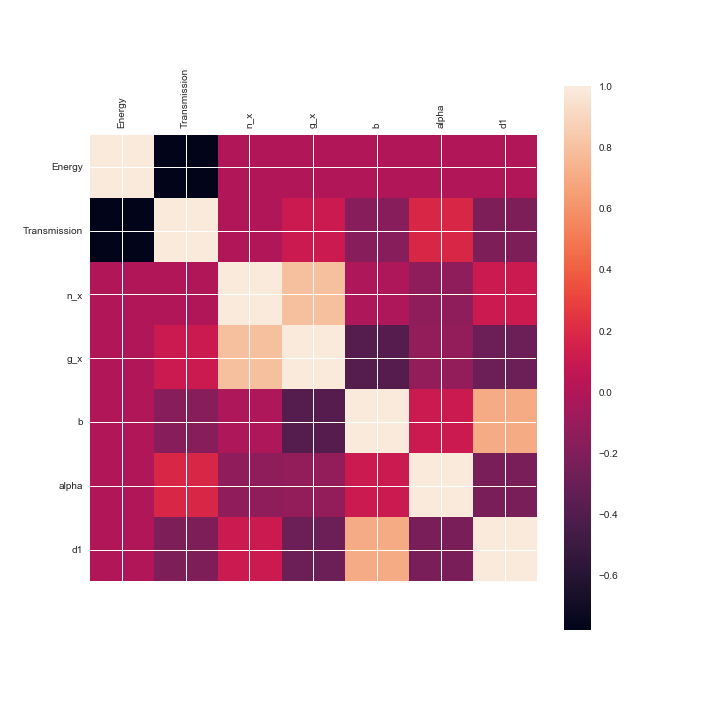
\includegraphics[width=300pt]{figuras/correlacao.png}
  \caption{Correlação das propriedades}
  \label{fig:correlacao}
\end{figure}

\subsection{Inicialização dos pesos sinápticos}

Após identificar os diversos parâmetros que descrevem as configurações físicas e influenciam nas propriedades eletrônicas em nanofita de grafeno, este trabalho faz o uso de rede neural artificial para descrever quantitativelmente os efeitos destes parâmetros na transmissão por vale. Detalhes destas atividades estão explicados nas seguintes sessões.

\section{Conjunto de dados e pré-processamento}
Os dados foram obtidos a partir de cálculos de  transporte eletrônico em nanofitas de grafeno com um número definido de deformações gaussianas. Eles foram estruturados em arquivos com extensões .txt e .dat. Estes arquivos foram então processados para gerar um único conjunto de dados que foi usado para treinar a rede neural artificial.
Cada arquivo .txt contém diversos parâmetros que descrevem as diferentes configuração físicas de nanofita de grafeno. Por exemplo, o arquivo com os seguintes pares de chave-valor foram analisados e a chave $n_y$ (número de átomos na direção vertical) com valor 70 resultou numa coluna cujos valores são iguais a 70. O mesmo foi feito para as chaves $n_x$ (número de átomos na direção vertical) com valor 2001 e $g_x$ (número de deformações gaussianas na direção horizontal) com valor 50.

\begin{table}[H]
\begin{minipage}{0.5\linewidth}
\caption{Conjunto chave-valor de configuração pré-processamento.}
\label{tab:chave_valores_preprocessamento}
\centering
\begin{tabular}{c|c}
\toprule
\textbf{Chave} & \textbf{Valor} \\
\midrule
\bm{$n_y$} & $70$    \\
\bm{$n_x$} & $2001$  \\
\bm{$g_x$} & $50$    \\
\textbf{b}   & $6ab$   \\
\bm{$d_1$}  & $20\sqrt{3}ac$   \\
\textbf{alpha}  & $22.2$\% \\
\bottomrule % <-- Bottomrule here
\end{tabular}
\end{minipage}
\begin{minipage}{0.5\linewidth}
\caption{Conjunto chave-valor de configuração pós processamento.}
\label{tab:chave_valores_posprocessamento}
\centering
\begin{tabular}{c|c}
\toprule
\textbf{Chave} & \textbf{Valor} \\
\midrule
\bm{$n_y$} & 70    \\
\bm{$n_x$} & 2001  \\
\bm{$g_x$} & 50    \\
\textbf{b}   & $0,0852$   \\
\bm{$d_1$}  & $4,919$   \\
\textbf{alpha}  & $0.222$\% \\
\bottomrule % <-- Bottomrule here
\end{tabular}
\end{minipage}
\end{table}

O mesmo foi feito com a chave b (desvio padrão das bases das deformações gaussianas) com o valor $6*ac$, mas um cálculo adicional foi feito devido a dependência no valor de $ac$ que é uma constante de distância entre os átomos de carbono valor $0.142nm$. Neste caso, a chave $b$ resultou numa coluna cujos valores são iguais a $6*0.142nm = 0,0852$. A chave $d1$ (distância entre cada deformação gaussiana) com o valor $20*\sqrt{3}*ac$ resultou em uma coluna cujos valores são iguais a $20*\sqrt{3}*0.142nm=4,919$. A chave $alpha$ (parâmetro de pressão da gaussiana) com o valor $22.2\%$ resultou numa coluna com valores iguais a $0.222$.

Um pouco de informação sobre o conjunto de dados:

\begin{table}[H]
    \begin{center}
    \caption{Descrição das propriedades envolvidas no experimento}
    \label{tab:Descrição das propriedades do grafeno}
    \resizebox{16cm}{!}{
    \begin{tabular}{ l | l }
    \toprule
	\textbf{Propriedade} & \textbf{Descrição} \\ 
	\midrule
    \bm{$n_x$} & número de átomos no eixo X, ou seja, é o comprimento da nanofita \\
    \bm{$n_y$} & número de átomos no eixo Y, ou seja, é a largura da nanofita  \\
    \bm{$g_x$} & número de deformações gaussianas ao longo do eixo X na nanofita de grafno \\
    \bm{$d_1$} & distância os centros de deformações gaussianas vizinhas na nanofita de grafeno \\
    \textbf{b} & largura das deformações gaussiana \\
    \textbf{alpha} & relação entre a altura e a largura da deformações gaussianas, ou seja, $\alpha = (A/b)^2$. Está relacionado com o \textit{strain} produzido por uma deformação gaussiana \\
    \textbf{Energy} & energia dos elétrons incidentes \\
    \textbf{Conductance} & condutância elétrica $G(2e^2/h)$ \\
    \textbf{Transmission} & probabilidade de transmissão por vale \\
    \bottomrule % <-- Bottomrule here
    \end{tabular}
    }
    \end{center}
\end{table}

Os dados foram estatisticamente descritos abaixo:

\begin{table}[h!]
  \begin{center}
    \caption{Análise estatística dos dados.}
    \label{tab:analise_estatistica_dados}
    \resizebox{16cm}{!}{
    \begin{tabular}{l | S | S | S | S | S | S | S | S | S}
      \toprule
      \textbf{Function} & \textbf{Energy} & \textbf{Conductance} & \textbf{Transmission} & \bm{$n_x$} & \bm{$n_y$} & \bm{$g_x$} & \textbf{b} & \textbf{alpha} & \bm{$d_1$} \\
      \midrule
	count & 59000.00 & 59000.00 & 59000.00 & 59000.00 & 59000.00 & 59000.00 & 59000.00 & 59000.00 & 59000.00 \\
	mean & 0.25 & 8.28 & 0.67 & 1257.76 & 73.81 & 12.13 & 3.06 & 14.34 & 11.64 \\ 
	std & 0.14 & 7.39 & 0.18 & 769.00 & 20.94 & 8.61 & 0.59 & 12.88 & 2.83 \\ 
	min & 0.001 & 0.60 & 0.49 & 40.00 & 20.00 & 0.00 & 0.85 & 0.00 & 4.90 \\ 
	0.25 & 0.12 & 2.11 & 0.53 & 801.00 & 70.00 & 7.00 & 3.12 & 1.00 & 11.07 \\ 
	0.5& 0.25 & 6.33 & 0.57 & 1145.00 & 70.00 & 11.00 & 3.12 & 13.00 & 11.07 \\ 
	0.75 & 0.37 & 12.78 & 0.73 & 1801.00 & 70.00 & 17.00 & 3.12 & 25.00 & 11.07 \\ 
	max & 0.50 & 48.92 & 1.00 & 3601.00 & 150.00 & 60.00 & 4.54 & 40.00 & 22.13 \\ 
      \bottomrule % <-- Bottomrule here
    \end{tabular}
    }
  \end{center}
\end{table}



% \section{Centralizar as variáveis de entrada}
% \section{Normalização dos dados}
% \section{Descorrelacionar variáveis de entrada}
% \section{Definição da função de ativação}
% \section{Escalar os dados de saída para o intervalo da função de ativação}
% \section{Inicialização dos pesos}
% \section{Uso de gradiente conjugado para regressão}


% A rede neural calcula uma função $M( Zˆp , W )$, onde $Z^p$ é o p-ésimo padrão de entrada, e $W$ representa o conjunto de parâmetros ajustáveis no sistema. A função de custo  $E^p=\frac{1}{2}(D^p,M(Z^p,W))^2$ mede a discrepância entre a saída ``correta'' ou esperada $D^p$ para o padrão de entrada $Z^p$ e a saída produzida pelo sistema. A função de custo médio $E_{treino}(W)$ é a média dos erros $E^{p}$ sobre um conjunto de pares $\{(D^1,Z^1),...(D^P,Z^P)\}$. A performance é estimada em um conjunto de dados disjunto do conjunto de dados de treinamento, chamado conjunto de teste. A função de custo mais comumente usada é erro quadrático médio.

As estratégias usadas nesta sessão buscam não somente minimizar a função de custo, mas melhorar a capacidade da rede neural de generalizar, isto é, de predizer valores para padrões não previamente apresentados à rede neural.

$$E_{treino}=\frac{1}{P} \sum_{p=1}^P E^p$$ 

Uma vez que rede neural artificial foi usada neste experimento, os dados precisam ser preparados para tal.
A maioria dos valores são maiores que 1, portanto os valores foram escalados no intervalo $[-0.9, 0.9]$ de forma a acelerar o processo de treinamento da RNA.

Os dados escalados estão estatisticamente descritos abaixo:

\begin{figure}
    \centering
    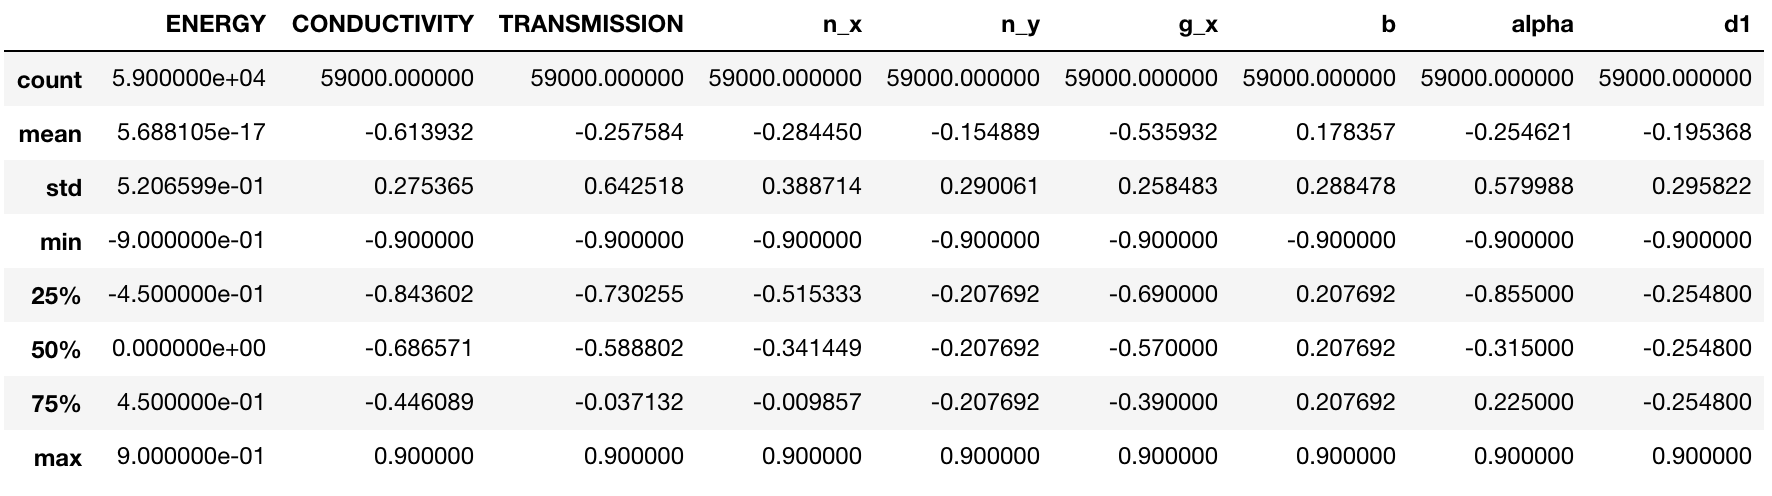
\includegraphics[width=350px]{figuras/scaled_data_summary.png}
    \caption{Descrição estatística dos dados escalados}
    \label{fig:Scaled data summary}
\end{figure}

\begin{figure}
    \centering
    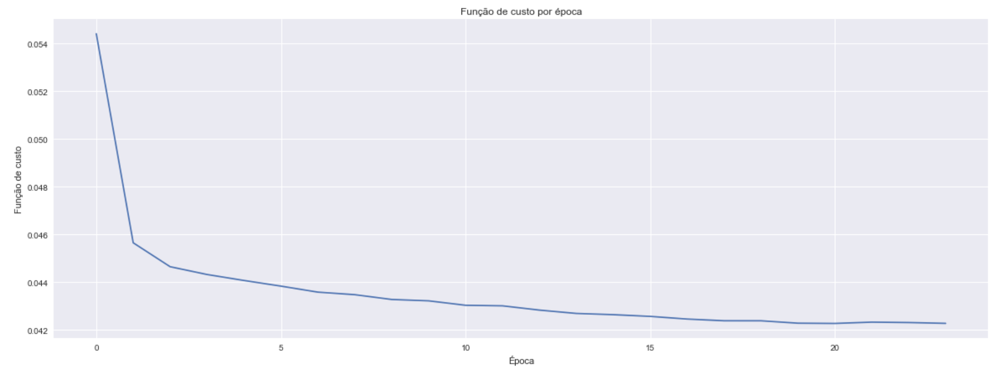
\includegraphics[width=350px]{figuras/erro_por_epoca.png}
    \caption{Função de erro por época de treinamento}
    \label{fig:Loss function per epoch}
\end{figure}

Cada arquivo .dat contém três colunas: energia($E/t$), condutância elétrica ($G(2e^2)/h)$) e transmissão por vale.

\sisetup{
  round-mode          = places, % Rounds numbers
  round-precision     = 3, % to 2 places
}

\begin{table}[h!]
    \begin{center}
    \caption{Análise de $R^2$ e RMSE por conjunto de parâmetros da MLP; $\eta$: Taxa de aprendizado; N: Neurônios na camada oculta; C: Condutância; T: Transmissão; val: validação; tre: treino; tes: teste.}
    \label{tab:analise_performance_mlp.}
    \resizebox{16cm}{!}{
    \begin{tabular}{ r | S |  S | S | S | S | S | S | S | S | S }
    \toprule
	\bm{$\eta$} & \textbf{N} & \textbf{R2 [tre]} & \textbf{RMSE C. [tre]} & \textbf{RMSE T. [tre]} & \textbf{R2 [val]} & \textbf{RMSE C. [val]} & \textbf{RMSE T. [val]} & \textbf{R2 [tes]} & \textbf{RMSE C. [tes]} & \textbf{RMSE T. [tes]} \\ 
	\midrule
0.01 & 50                         & 0.851880        & 0.075278                     & 0.274369                      & 0.847142           & 0.078587                        & 0.280333                         & 0.847591       & 0.077651                    & 0.278660                     \\
0.01 & 10                         & 0.853864        & 0.074270                     & 0.272525                      & 0.844657           & 0.079864                        & 0.282602                         & 0.843599       & 0.079685                    & 0.282286                     \\
0.01 & {(10, 10, 10)}               & 0.859360        & 0.071477                     & 0.267351                      & 0.859130           & 0.072423                        & 0.269116                         & 0.859277       & 0.071698                    & 0.267764                     \\
0.10 & 10                         & 0.859430        & 0.071441                     & 0.267285                      & 0.855857           & 0.074106                        & 0.272224                         & 0.860639       & 0.071004                    & 0.266465                     \\
0.10 & 50                         & 0.860539        & 0.070878                     & 0.266229                      & 0.853301           & 0.075420                        & 0.274627                         & 0.852997       & 0.074897                    & 0.273673                     \\
0.01 & {(10, 10)}                   & 0.864723        & 0.068751                     & 0.262205                      & 0.859285           & 0.072344                        & 0.268968                         & 0.858999       & 0.071839                    & 0.268028                     \\
0.01 & {(50, 50)}                   & 0.867618        & 0.067280                     & 0.259383                      & 0.860371           & 0.071785                        & 0.267928                         & 0.860841       & 0.070901                    & 0.266272                     \\
0.01 & {(50, 50, 50)}               & 0.875364        & 0.063343                     & 0.251681                      & 0.863935           & 0.069953                        & 0.264486                         & 0.865086       & 0.068738                    & 0.262179                     \\
0.10 & {(50, 50)}                   & 0.875471        & 0.063289                     & 0.251572                      & 0.864361           & 0.069734                        & 0.264072                         & 0.865918       & 0.068314                    & 0.261370                     \\
0.10 & {(10, 10, 10)}               & 0.877688        & 0.062162                     & 0.249323                      & 0.864821           & 0.069497                        & 0.263624                         & 0.865710       & 0.068420                    & 0.261572                     \\
0.10 & {(10, 10)}                   & 0.880147        & 0.060912                     & 0.246804                      & 0.860660           & 0.071637                        & 0.267650                         & 0.871035       & 0.065707                    & 0.256334                     \\
0.10 & {(50, 50, 50)}               & 0.894069        & 0.053837                     & 0.232028                      & 0.875658           & 0.063926                        & 0.252836                         & 0.872585       & 0.064917                    & 0.254789      \\           
    \bottomrule % <-- Bottomrule here
    \end{tabular}
    }
    \end{center}
\end{table}

\begin{table}[H]
\centering
\caption{Parâmetros que definem a estrutura da MLP já treinada.}
\label{parametros_rede_treinada}
\begin{tabular}{ r | l }
\toprule
\textbf{Especificação} & \textbf{Valor} \\
\midrule
Rede Neural & Perceptron de multiplas camadas \\
Função de ativação & tangente hiperbólica \\
Taxa de aprendizado & 0.10 \\
Momentum & 0.90 \\
Número de camadas ocultas & 1.00 \\
Número de nós na camada oculta & {(50,50,50)} \\
Número de nós na camada de entrada  & 6.00 \\
Número de nós na camada de saída & 1.00 \\
Algorítimo  & gradiente estocástico descendente \\
\bottomrule
\end{tabular}
\end{table}

\section{Modelagem de rede neural artificial e parametrização}
Na primeira etapa os dados pré-processados foram ordenados de foram aleatória e divididos em conjunto de treinamento, validação e teste. A porcentagem de observações por conjunto é de 60\%, 20\% e 20\%, para os conjuntos de treinamento, validação e teste, respectivamente. O conjunto de treinamento foi usado para treinar a Rede Neural Artificial (RNA). Os  dados de validação foi usado em conjunto com o dados de treinamento para determinar quando interromper o processo de aprendizado, de modo que o modelo resultante exibisse boas métricas de generalização. Os dados de teste permitem a avaliação das capacidades de predição do modelo de RNA. A RNA foi avaliada usando como
critérios de desempenho o erro quadrado médio (MSE) e o coeficiente de determinação ($R^2$) sobre os conjuntos de dados de treinamento e teste.

\todo{Rever esta parte}

A seguinte etapa se refere a configuração e a otimização da arquitetura de RNA. O modelo de RNA foi projetado com três camadas: uma camada de entrada, uma
camada oculta e uma camada de saída. De um modo geral, uma camada oculta é suficiente para a maioria dos problemas práticos de regressão, portanto, apenas uma camada oculta foi usada neste estudo. O desempenho da RNA foi testado com mais de uma camada oculta.
A quantidade de nós na camada de entrada e saída da RNA foram definidos de acordo com o número de fatores/atributos de entrada e o número de variáveis a serem previstas. A camada de entrada tem nove nós que representam as seis chaves supracitadas além das propriedades energia, condutância elétrica e transmissão por vale. Uma busca exaustiva foi realizada para determinar o número ideal de neurônios na camada oculta, a taxa de aprendizado, o algorítmo de aprendizado, a função de ativação / saída, momentum e alpha de acordo com os critérios de desempenho supracitados.

% \section{Análise de desempenho e erro da rede neural}

% \section{Análise gráfica dos erros nos subconjuntos de treino, validação e teste}

\section{Arquitetura da rede neural treinada}

A estrutura final do modelo da RNA possui 50 neurônios em cada camada oculta. A função de ativação da camada oculta e na camada de saída do modelo é a função tangente hiperbólica. O processo de treinamento foi conduzido utilizando o algoritmo padrão de retropropagação (gradiente estocástico descendente) como procedimento de otimização, com pesos atualizados a cada vez que o conjunto completo de dados de treinamento foi considerado.
O modelo de RNA obteve um bom desempenho nos dados de treinamento / validação / teste, com um valor de $R^2$ de ~ $0.909$ para cada. A RNA desempenhou satisfatoriamente para todo o conjunto de dados. Deve-se perceber que esse modelo de RNA não considera outros fatores que possam afetar os valores de transmissão por vale. O conjunto de dados que suporta o modelo de RNA é limitado às condições investigadas neste experimento. Devido à sua natureza orientada por dados, o modelo de RNA pode ser melhorado progressivamente, treinando-o com mais dados observados.

% PRE-PROCESSAMENTO
% 1-Discretização
% 2-Normalização/Scale the data
% MODELAGEM DE REDE NEURAL
% 